% !TEX encoding = UTF-8
% !TEX TS-program = pdflatex
% !TEX root = ../tesi.tex

%**************************************************************
\section{Sprint 2}
\label{sec:sprint2}
%**************************************************************

Durante il secondo sprint ho redatto la versione conclusiva del documento relativo alle user stories, approvato poi dal mio relatore esterno.

\noindent All'inizio di ogni capitolo relativo a uno sprint indicherò le user stories su cui andrò a lavorare.

Per concludere la settimana ho lavorato a dei piccoli bugfix e features, anche per familiarizzare con la web app e i pattern utilizzati.
In particolare ho: 
\begin{itemize}
  \item sistemato un problema con la immagine nella pagina di login, che non si rimpiccioliva nel caso la finestra facesse lo stesso;
  \item fatto sì che, nella pagina utente, nel caso quest'ultimo non la avesse inserita, venissero mostrate le iniziali dell'utente invece che nulla;
  \item implementato una finestra di dialogo che semplicemente chiede di confermare o annullare un'azione.
\end{itemize}

Seppure i primi due problemi fossero molto semplici e risolvibili principalmente con del codice CSS, creare la finestra di dialogo mi è stato utile sia a familiarizzare con React, che non avevo mai utilizzato, ma anche a capire meglio come fosse strutturata la applicazione.\\

\subsection{Casi d'uso individuati}
Ho inoltre creato dei diagrammi UML dei casi d'uso, di cui i più significativi sono elencati di seguito.

\begin{figure}[bp!]
	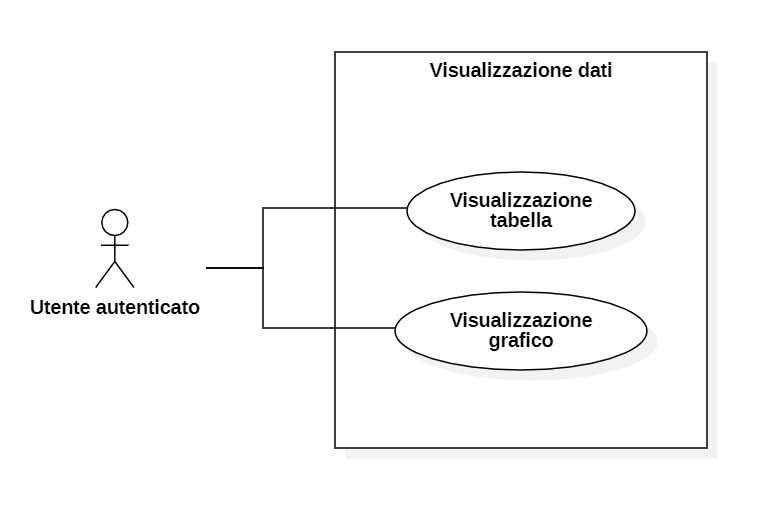
\includegraphics[width = \textwidth*\real{0.7}]{immagini/usecase/visualizzazione_dati.png}
	\caption{Use case per la visualizzazione dati}
	\label{fig:uc_vis_dati}
\end{figure}

\begin{figure}[bp!]
	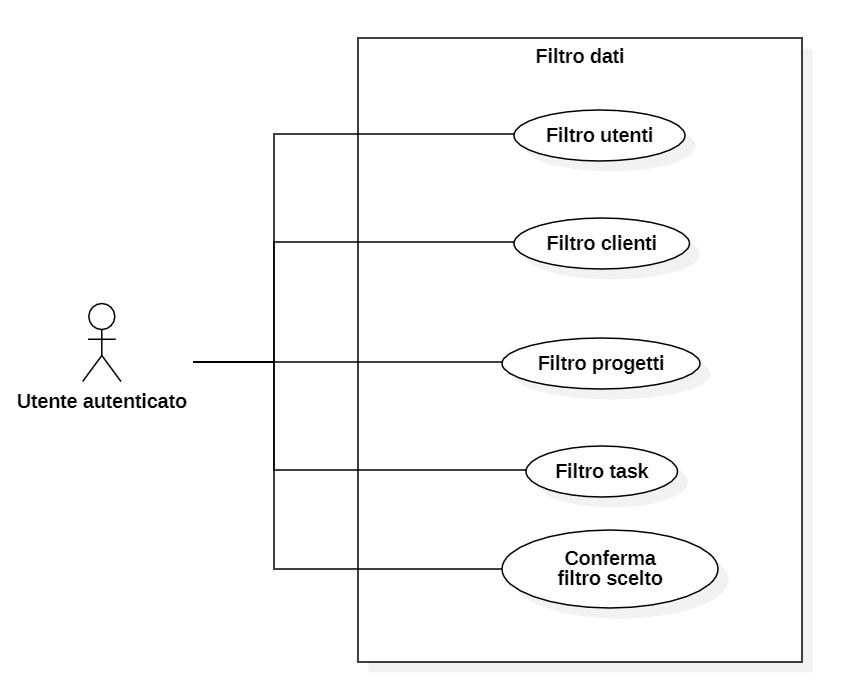
\includegraphics[width = \textwidth*\real{0.7}]{immagini/usecase/filtro_dati.png}
	\caption{Use case per il filtro dati}
	\label{fig:uc_filtro}
\end{figure}

\begin{figure}[bp!]
	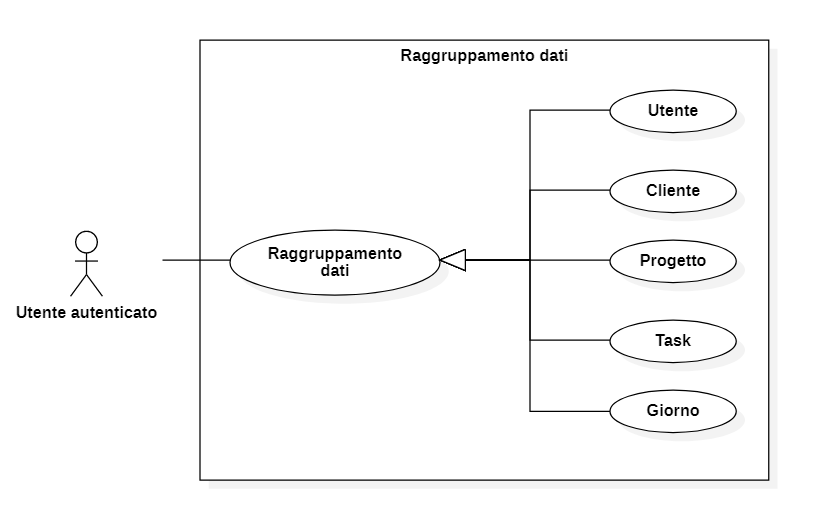
\includegraphics[width = \textwidth*\real{0.7}]{immagini/usecase/raggruppamento_dati.png}
	\caption{Use case per la visualizzazione dati}
	\label{fig:uc_raggruppamento}
\end{figure}

\begin{figure}[bp!]
	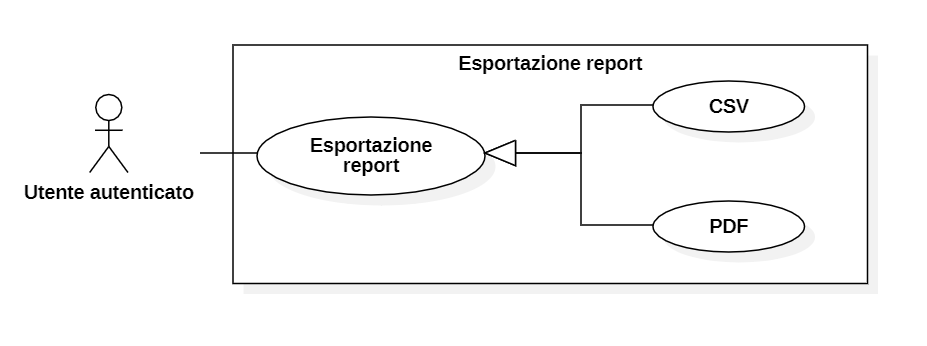
\includegraphics[width = \textwidth*\real{0.7}]{immagini/usecase/esportazione_report.png}
	\caption{Use case per la visualizzazione dati}
	\label{fig:uc_export}
\end{figure}